\documentclass[a4paper]{article}

% --- Основные пакеты ---
\usepackage{graphicx}     % картинки
\usepackage{geometry}     % поля страницы
\usepackage{hyperref}     % гиперссылки
\usepackage{amsmath}      % математика
\usepackage{amssymb}      % математические символы
\usepackage{float}        % [H] позиционирование фигур
\usepackage[T2A]{fontenc} % кириллица
\usepackage[utf8]{inputenc} % кодировка UTF-8
\usepackage[russian]{babel} % многоязычность
\usepackage{caption}      % настройка подписей
\usepackage{longtable}    % длинные таблицы
\usepackage{array}        % расширенные таблицы
\usepackage{multirow}     % объединение строк в таблицах

% --- Настройка страницы ---
\geometry{top=1.5cm, bottom=1.5cm, left=3cm, right=1.5cm}

\renewcommand{\thesubsection}{\arabic{subsection}.}

% --- Настройка гиперссылок ---
\hypersetup{
    colorlinks,
    linkcolor=black,
    urlcolor=blue,
    citecolor=black
}

% --- Настройка подписей ---
\renewcommand{\figurename}{Рис.}
\captionsetup{labelsep=period}

\begin{document}

% --- Титульная страница ---
\centering
Министерство науки и высшего образования Российской Федерации\\
Федеральное государственное автономное образовательное учреждение\\
высшего образования\\
«Южно-Уральский государственный университет\\
(национальный исследовательский университет)»\\
Институт естественных и точных наук

\setlength{\parskip}{7.5cm}

Отчет\\
Лабораторная работа №8.\\
Решение обыкновенных дифференциальных уравнений.

\setlength{\parskip}{6.5cm}

\raggedleft
\begin{minipage}{0.345\textwidth}
\raggedright
Выполнил: студент группы ЕТ-210\\
Тельнов С.М.\\
Проверил: преподаватель кафедры ВМ\\
Стариков Я.Е.
\end{minipage}

\setlength{\parskip}{6cm}

\centering
Челябинск — 2026

\setlength{\parskip}{0pt plus 1pt}
\newpage

% --- Содержание ---
\centering
\textbf{Краткое содержание}
\begin{itemize}
    \setlength{\parskip}{0.4cm}
    \item \hyperref[sec:theory]{\text{Теоретическая часть} \dotfill \pageref{sec:theory}}
    \item \hyperref[sec:practice]{\text{Практическая часть} \dotfill \pageref{sec:practice}}
    \item \hyperref[sec:conclusion]{\text{Вывод} \dotfill \pageref{sec:conclusion}}
\end{itemize}

\setlength{\parindent}{1.5em}

\raggedright

% --- Теоретическая часть ---
\section*{\centering\fontsize{14pt}{0pt}\selectfont\textbf{Теоретическая часть}\label{sec:theory}}

\section{Цель работы}
Изучение численных методов решения задачи Коши для обыкновенных дифференциальных уравнений (ОДУ) и их систем (СОДУ). Получение практических навыков построения алгоритмов с фиксированным и адаптивным выбором шага интегрирования, а также проведение сравнительного анализа их точности и вычислительной эффективности.

\section{Постановка задачи Коши}
Численное решение дифференциальных уравнений заключается в нахождении приближённых значений искомой функции на заданной сетке узлов аргумента $t$.

\subsection{Задача Коши для одного ОДУ первого порядка}
Задача формулируется как нахождение функции $y(t)$, удовлетворяющей уравнению и начальному условию на отрезке $t \in [t_0, top_K]$:
\begin{equation}
\begin{cases}
y^{\prime} = f(t, y), \\
y(t_0) = y_0.
\end{cases}
\label{eq:ode}
\end{equation}

\subsection{Задача Коши для системы двух ОДУ первого порядка}
Задача формулируется как нахождение функций $x(t)$ и $y(t)$, удовлетворяющих системе уравнений и начальным условиям на отрезке $t \in [t_0, t_K]$:
\begin{equation}
\begin{cases}
x^{\prime} = f(t, x, y), \\
y^{\prime} = \varphi(t, x, y),
\end{cases}
\label{eq:system}
\end{equation}
с начальными условиями: $x(t_0) = x_0, \, y(t_0) = y_0$.

\section{Численные методы с фиксированным шагом}
При фиксированном шаге $h = \Delta t$ расчетная сетка строится равномерно: $t_{n+1} = t_n + h$.

\subsection{Одношаговые методы}
В одношаговых методах для вычисления значения решения в точке $t_{n+1}$ используется информация о решении только в предыдущей точке $t_n$.

\begin{enumerate}
    \item \textbf{Явный метод Эйлера (1-й порядок точности):}
    Аппроксимирует производную наклоном интегральной кривой в начале шага:
    \begin{equation}
    y_{n+1} = y_n + h \cdot f(t_n, y_n).
    \end{equation}
    
    \item \textbf{Модифицированный метод Эйлера (2-й порядок точности):}
    Использует схему прогноза и коррекции для повышения точности за счет усреднения производных:
    \begin{align}
    \tilde{y}_{n+1} &= y_n + h \cdot f(t_n, y_n) \quad \text{(прогноз)}, \\
    y_{n+1} &= y_n + \frac{h}{2} \Big[ f(t_n, y_n) + f(t_{n+1}, \tilde{y}_{n+1}) \Big] \quad \text{(коррекция)}.
    \end{align}
    
    \item \textbf{Метод Рунге-Кутты (4-й порядок точности):}
    Обеспечивает высокую точность $O(h^4)$ на отрезке за счет четырехкратного вычисления правой части уравнения внутри каждого шага:
    \begin{equation}
    y_{n+1} = y_n + \frac{h}{6}(k_1 + 2k_2 + 2k_3 + k_4),
    \end{equation}
    где $k_1 = f(t_n, y_n)$, \ $k_2 = f\left(t_n + \frac{h}{2}, y_n + \frac{h}{2}k_1\right)$, \ $k_3 = f\left(t_n + \frac{h}{2}, y_n + \frac{h}{2}k_2\right)$, \ $k_4 = f(t_n + h, y_n + hk_3)$.
\end{enumerate}

\subsection{Многошаговые методы (методы Адамса)}
Многошаговые методы используют предысторию процесса — значения решения в нескольких предшествующих узлах ($t_n, t_{n-1}, \dots$), что позволяет повысить порядок точности без увеличения числа вычислений функции правой части.

\begin{enumerate}
    \item \textbf{Явный метод Адамса (Башфорта):}
    Экстраполяционный метод. Двухшаговая схема (2-й порядок точности) имеет вид:
    \begin{equation}
    y_{n+1} = y_n + h \left( \frac{3}{2}f(t_n, y_n) - \frac{1}{2}f(t_{n-1}, y_{n-1}) \right).
    \end{equation}
    
    \item \textbf{Модифицированный метод Адамса (Предиктор-Корректор):}
    Сочетает в себе явный метод Адамса-Башфорта для построения предварительного прогноза решения и неявный метод Адамса-Мултона для его последующей коррекции. Для вычисления начальных (стартовых) точек многошаговых схем применяются одношаговые методы аналогичного порядка точности.
\end{enumerate}

\section{Методы с адаптивным выбором шага}
Методы с адаптивным (переменным) шагом динамически изменяют величину шага $h$ в процессе интегрирования на основе оценки локальной погрешности $\Delta$. Если $\Delta$ превышает заданную точность $\varepsilon$, текущий шаг отклоняется и вычисляется заново с меньшей величиной. Если $\Delta \ll \varepsilon$, величина шага для последующего этапа увеличивается.

\begin{enumerate}
    \item \textbf{Метод Рунге-Кутты-Мерсона:}
    Пятиэтапная модификация стандартного метода Рунге-Кутты, которая позволяет оценивать локальную погрешность четвертого порядка без существенных дополнительных затрат.
    
    \item \textbf{Метод Рунге-Кутты-Фельберга (РКФ45):}
    Основан на одновременном вычислении решений четвертого и пятого порядков точности с использованием общего набора коэффициентов. Разность между этими решениями служит прямой оценкой локальной погрешности.
    
    \item \textbf{Адаптивный модифицированный метод Эйлера:}
    Применяет алгоритм двойного пересчета (правило Рунге). На каждом этапе решение находится дважды: один раз с шагом $h$ и один раз двумя последовательными шагами по $h/2$. Оценка погрешности производится по величине расхождения полученных результатов.
\end{enumerate}

\newpage

% --- Практическая часть ---
\section*{\centering\fontsize{14pt}{0pt}\selectfont\textbf{Практическая часть}\label{sec:practice}}

\subsection*{Задача 1. Решение обыкновенного дифференциального уравнения}

Рассматривается задача Коши для ОДУ первого порядка:
\begin{equation}
y' = y \cdot \cos(t) + \sin(2t), \quad y(0) = 1, \quad t \in [0, 10].
\label{eq:task1}
\end{equation}

В качестве эталонного использовалось решение, полученное с помощью встроенной функции \texttt{solve\_ivp} библиотеки SciPy с параметрами \texttt{method='RK45'}, \texttt{max\_step=0.001}, \texttt{rtol=1e-9}, \texttt{atol=1e-12}. Эталонное значение: $y(10) = 0.829271207920$.

\subsection*{Задача 1.1. Методы с фиксированным шагом}

Для решения уравнения (\ref{eq:task1}) применялись пять численных методов с фиксированным шагом: явный метод Эйлера 1-го порядка, модифицированный метод Эйлера 2-го порядка, метод Рунге-Кутты 4-го порядка, явный метод Адамса 2-го порядка и предиктор-корректор Адамса. Для каждого метода подбирался шаг $h$, обеспечивающий погрешность $\le 10^{-4}$. Результаты представлены в таблице~\ref{tab:task1_fixed}.

\begin{table}[H]
\centering
\caption{Методы с фиксированным шагом для ОДУ (ошибка $\le 10^{-4}$)}
\label{tab:task1_fixed}
\begin{tabular}{|l|c|c|c|c|}
\hline
\textbf{Метод} & \textbf{$y(10)$} & \textbf{Шаг $h$} & \textbf{Ошибка} & \textbf{Шагов} \\
\hline
Эйлер 1-го порядка      & 0.8292078666 & $4.88\cdot10^{-5}$ & $6.33\cdot10^{-5}$ & 204\,800 \\
Модиф. Эйлер 2-го порядка & 0.8293344962 & $2.50\cdot10^{-2}$ & $6.33\cdot10^{-5}$ & 400 \\
Рунге-Кутта 4-го порядка  & 0.8292717508 & $1.00\cdot10^{-1}$ & $5.43\cdot10^{-7}$ & 100 \\
Явный Адамс 2-го порядка  & 0.8293692794 & $1.25\cdot10^{-2}$ & $9.81\cdot10^{-5}$ & 800 \\
Предиктор-корректор Адамса & 0.8292376296 & $6.25\cdot10^{-3}$ & $3.36\cdot10^{-5}$ & 1\,600 \\
\hline
\end{tabular}
\end{table}

Наилучший результат показал метод Рунге-Кутты 4-го порядка: для достижения требуемой точности потребовалось всего 100 шагов при максимальном шаге $h = 0.1$, а полученная ошибка ($5.43\cdot10^{-7}$) оказалась на два порядка ниже заданного порога. Метод Эйлера 1-го порядка, напротив, потребовал 204\,800 шагов при шаге $h = 4.88\cdot10^{-5}$, что в 2\,048 раз больше, чем у метода Рунге-Кутты 4-го порядка. Модифицированный метод Эйлера (400 шагов) и методы Адамса (800 и 1\,600 шагов) заняли промежуточное положение.

\subsection*{Задача 1.2. Методы с адаптивным шагом}

Для того же уравнения были применены три адаптивных метода: Рунге-Кутты-Мерсона, адаптивный модифицированный метод Эйлера и Рунге-Кутты-Фельберга (РКФ45). Результаты при точности $\varepsilon = 10^{-4}$ представлены в таблице~\ref{tab:task1_adaptive}.

\begin{table}[H]
\centering
\caption{Адаптивные методы для ОДУ}
\label{tab:task1_adaptive}
\begin{tabular}{|l|c|c|c|c|}
\hline
\textbf{Метод} & \textbf{$y(10)$} & \textbf{$\varepsilon$} & \textbf{Ошибка} & \textbf{Шагов} \\
\hline
Рунге-Кутта-Мерсон     & 0.8292712079 & $9.54\cdot10^{-11}$ & $2.41\cdot10^{-11}$ & 1\,549 \\
Адаптивный модиф. Эйлер & 0.8293535500 & $1.00\cdot10^{-4}$   & $8.23\cdot10^{-5}$  & 156 \\
РК-Фельберг 45         & 0.8293468893 & $5.00\cdot10^{-5}$   & $7.57\cdot10^{-5}$  & 34 \\
\hline
\end{tabular}
\end{table}

Метод РК-Фельберга 45 показал наименьшее количество шагов (34), что свидетельствует о высокой эффективности алгоритма адаптации шага. Метод Рунге-Кутты-Мерсона автоматически подобрал значение $\varepsilon$ до $9.54\cdot10^{-11}$, обеспечив наименьшую ошибку, однако ценой большего числа шагов (1\,549). Адаптивный метод Эйлера занял промежуточное положение (156 шагов).

\subsection*{Задача 1.3. Сравнение количества шагов}

Сводный анализ числа шагов (таблица~\ref{tab:task1_steps}) показывает существенное различие в вычислительной эффективности методов.

\begin{table}[H]
\centering
\caption{Сравнение количества шагов для ОДУ}
\label{tab:task1_steps}
\begin{tabular}{|l|c|}
\hline
\textbf{Метод} & \textbf{Шагов} \\
\hline
Эйлер 1-го порядка (фикс.)           & 204\,800 \\
Модиф. Эйлер 2-го порядка (фикс.)    & 400 \\
Рунге-Кутта 4-го порядка (фикс.)     & 100 \\
Явный Адамс 2-го порядка (фикс.)     & 800 \\
Предиктор-корректор Адамса (фикс.)   & 1\,600 \\
Рунге-Кутта-Мерсон (адапт.)          & 1\,549 \\
Адаптивный модиф. Эйлер (адапт.)     & 156 \\
РК-Фельберг 45 (адапт.)              & 34 \\
\hline
\texttt{solve\_ivp} (эталон)          & 10\,002 \\
\hline
\end{tabular}
\end{table}

Метод Эйлера 1-го порядка потребовал наибольшего числа шагов (204\,800), что связано с низким порядком точности. Метод Рунге-Кутты 4-го порядка и адаптивные методы (особенно РКФ45) оказались наиболее эффективными. Эталонное решение \texttt{solve\_ivp} использовало 10\,002 шага, что обусловлено крайне малым максимальным шагом ($h_{max} = 0.001$), заданным для обеспечения высокой точности.

\subsection*{Задача 2. Решение системы обыкновенных дифференциальных уравнений}

Рассматривается задача Коши для системы двух ОДУ:
\begin{equation}
\begin{cases}
x' = (2 - 2.5y) \cdot x,\\
y' = (x - 2) \cdot y^2,
\end{cases}
\quad x(0) = y(0) = 1, \quad t \in [0, 10].
\label{eq:task2}
\end{equation}

Эталонное решение получено с помощью \texttt{solve\_ivp}:
\begin{itemize}
    \item $x(10) = 3.333980190255$;
    \item $y(10) = 1.128292387155$;
    \item число шагов: 10\,002.
\end{itemize}

\subsection*{Задача 2.1. Методы с фиксированным шагом}

Для системы (\ref{eq:task2}) применялись те же пять методов с фиксированным шагом. Результаты при точности $\le 10^{-4}$ представлены в таблице~\ref{tab:task2_fixed}.

\begin{table}[H]
\centering
\caption{Методы с фиксированным шагом для СОДУ}
\label{tab:task2_fixed}
\begin{tabular}{|l|c|c|c|c|c|}
\hline
\textbf{Метод} & \textbf{$x(10)$} & \textbf{$y(10)$} & \textbf{Шаг $h$} & \textbf{Ошибка} & \textbf{Шагов} \\
\hline
Эйлер 1-го порядка      & 3.3340429262 & 1.1282846360 & $1.53\cdot10^{-6}$ & $6.32\cdot10^{-5}$ & 6\,553\,600 \\
Модиф. Эйлер 2-го порядка & 3.3339071080 & 1.1283462851 & $3.13\cdot10^{-3}$ & $9.08\cdot10^{-5}$ & 3\,200 \\
Рунге-Кутта 4-го порядка  & 3.3339894878 & 1.1282850167 & $5.00\cdot10^{-2}$ & $1.19\cdot10^{-5}$ & 200 \\
Явный Адамс 2-го порядка  & 3.3339461573 & 1.1283228139 & $1.56\cdot10^{-3}$ & $4.57\cdot10^{-5}$ & 6\,400 \\
Модиф. Адамс (пред.-кор.) & 3.3340603751 & 1.1283022301 & $6.25\cdot10^{-3}$ & $8.08\cdot10^{-5}$ & 1\,600 \\
\hline
\end{tabular}
\end{table}

Для системы ОДУ наблюдается та же закономерность, что и для одного уравнения. Метод Эйлера 1-го порядка потребовал более 6.5 миллионов шагов, что делает его практически неприменимым для данной задачи. Метод Рунге-Кутты 4-го порядка вновь показал наилучший результат среди методов с фиксированным шагом (200 шагов, ошибка $1.19\cdot10^{-5}$).

\subsection*{Задача 2.2. Адаптивный метод РК-Фельберга 45}

Для уточнения решения применялся метод РК-Фельберга 45 с различными значениями допуска $tol$. Результаты представлены в таблице~\ref{tab:task2_adaptive}.

\begin{table}[H]
\centering
\caption{Метод РК-Фельберга 45 для СОДУ с различным $tol$}
\label{tab:task2_adaptive}
\begin{tabular}{|c|c|c|c|c|}
\hline
\textbf{$tol$} & \textbf{$x(10)$} & \textbf{$y(10)$} & \textbf{Ошибка} & \textbf{Шагов} \\
\hline
$10^{-4}$ & 3.3317270498 & 1.1289676998 & $2.35\cdot10^{-3}$ & 52 \\
$10^{-5}$ & 3.3338165808 & 1.1283014847 & $1.64\cdot10^{-4}$ & 75 \\
$10^{-6}$ & 3.3339750914 & 1.1282857360 & $8.38\cdot10^{-6}$ & 107 \\
$10^{-7}$ & 3.3339803388 & 1.1282912992 & $1.10\cdot10^{-6}$ & 136 \\
\hline
\end{tabular}
\end{table}

При ужесточении допуска точность закономерно возрастает, однако растёт и число шагов. Оптимальным представляется выбор $tol = 10^{-6}$, обеспечивающий ошибку $8.38\cdot10^{-6}$ при 107 шагах — это лучше, чем у метода Рунге-Кутты 4-го порядка с фиксированным шагом (200 шагов при ошибке $1.19\cdot10^{-5}$).

\subsection*{Задача 2.3. Графики решений}

На рисунке~\ref{fig:xt_yt} представлены графики $x(t)$ и $y(t)$, полученные различными методами, а на рисунке~\ref{fig:phase} — фазовая траектория $y(x)$.

\begin{figure}[H]
\centering
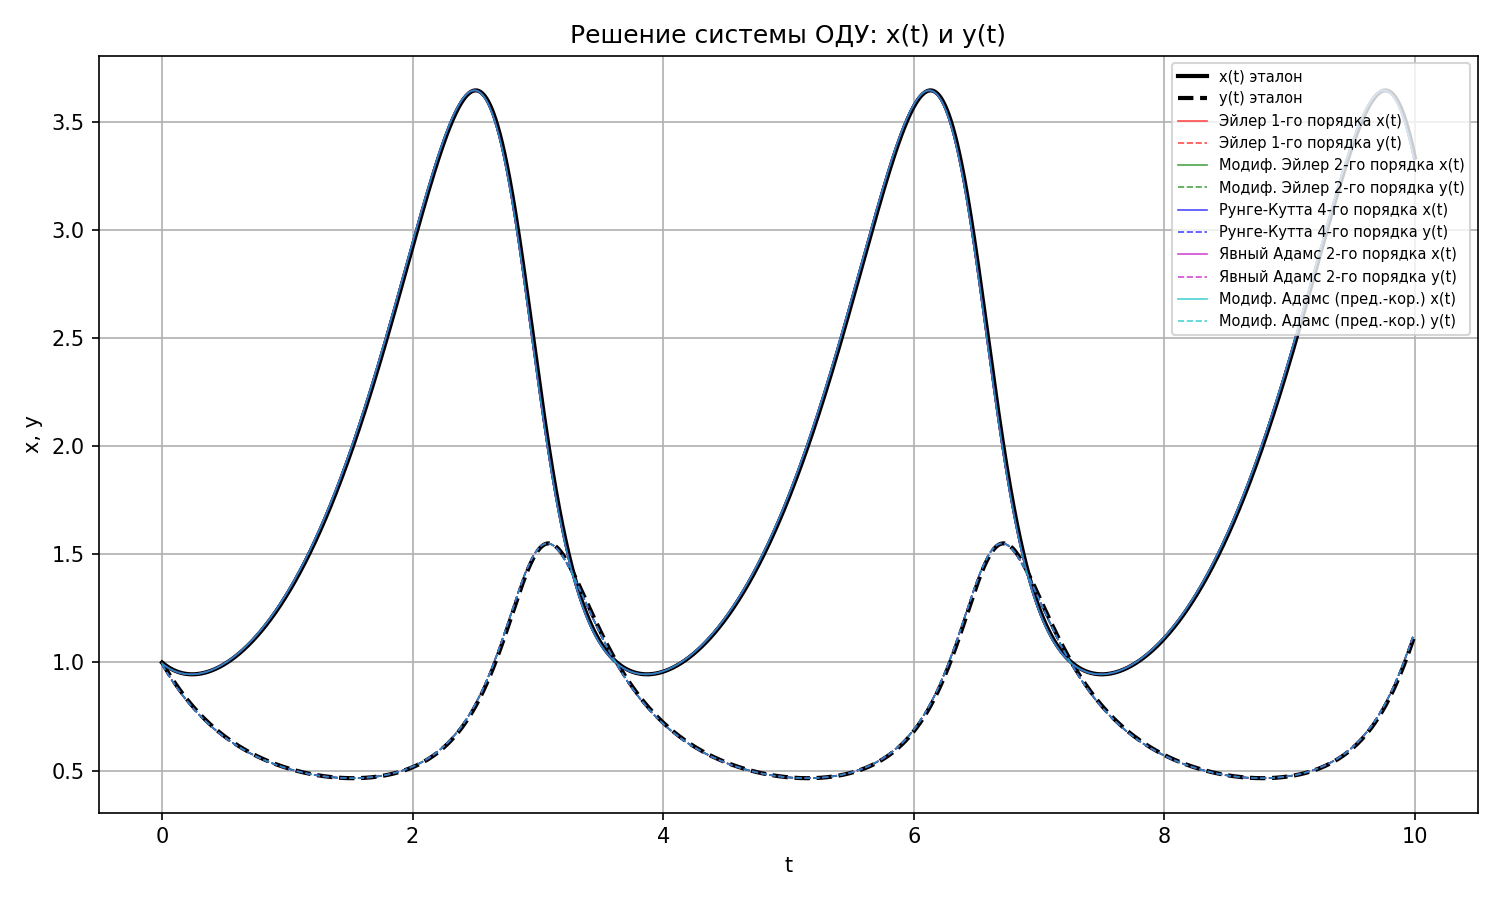
\includegraphics[width=0.95\textwidth]{../task2_xt_yt.png}
\caption{Графики $x(t)$ и $y(t)$ для системы ОДУ}
\label{fig:xt_yt}
\end{figure}

\begin{figure}[H]
\centering
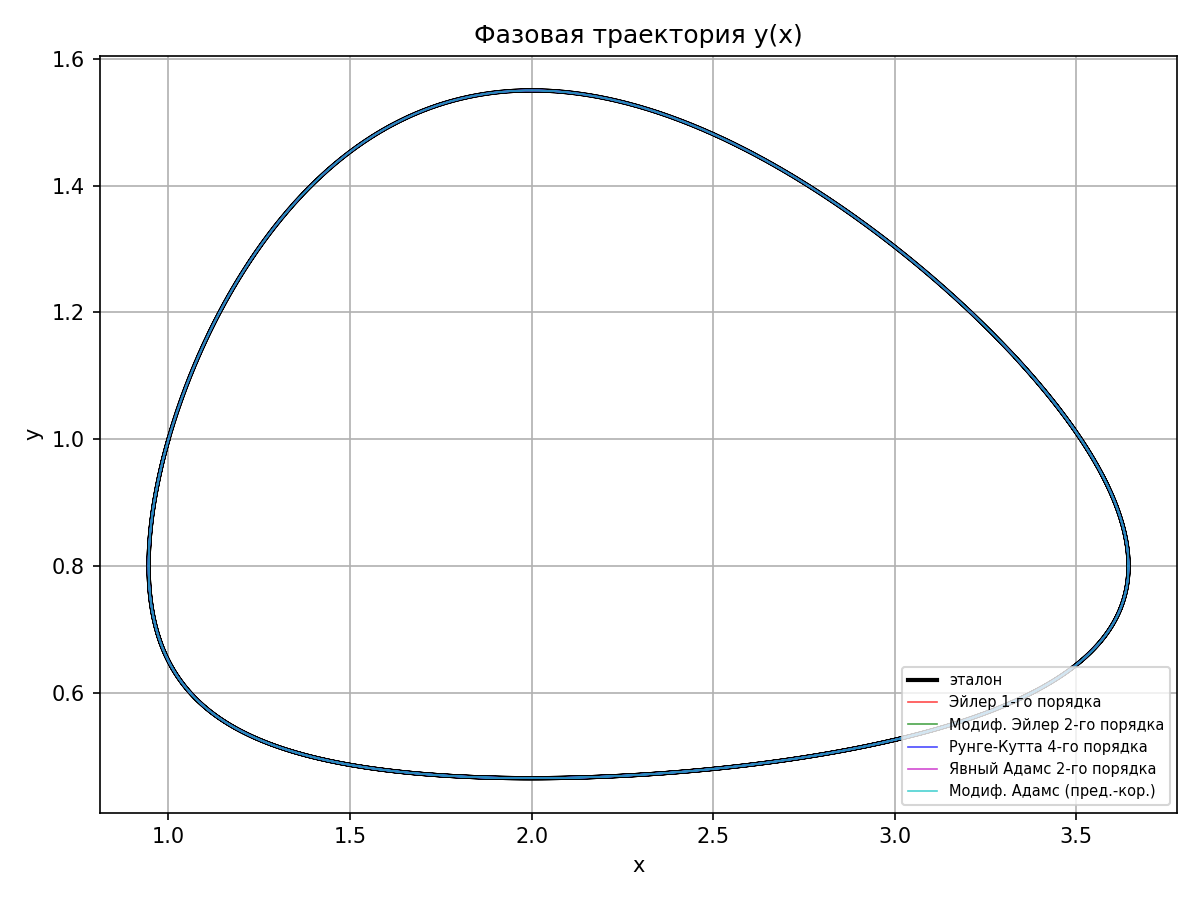
\includegraphics[width=0.75\textwidth]{../task2_phase.png}
\caption{Фазовая траектория $y(x)$}
\label{fig:phase}
\end{figure}

На графиках $x(t)$ и $y(t)$ видно, что решения, полученные различными методами, хорошо согласуются с эталонным. Фазовая траектория показывает, что система стремится к некоторому предельному циклу: значение $x(t)$ растёт и приближается к 3.33, а $y(t)$ стабилизируется около 1.13. Все численные методы корректно воспроизводят качественное поведение системы.

\subsection*{Задача 2.4. Сводка по количеству шагов}

Сравнительный анализ числа шагов для системы ОДУ (таблица~\ref{tab:task2_steps}) подтверждает выводы, сделанные для одного уравнения.

\begin{table}[H]
\centering
\caption{Сравнение количества шагов для СОДУ}
\label{tab:task2_steps}
\begin{tabular}{|l|c|}
\hline
\textbf{Метод} & \textbf{Шагов} \\
\hline
Эйлер 1-го порядка (фикс.)              & 6\,553\,600 \\
Модиф. Эйлер 2-го порядка (фикс.)       & 3\,200 \\
Рунге-Кутта 4-го порядка (фикс.)        & 200 \\
Явный Адамс 2-го порядка (фикс.)        & 6\,400 \\
Модиф. Адамс (пред.-кор.) (фикс.)       & 1\,600 \\
РК-Фельберг 45 ($tol = 10^{-6}$) (адапт.) & 107 \\
\hline
\texttt{solve\_ivp} (эталон)             & 10\,002 \\
\hline
\end{tabular}
\end{table}

Метод Эйлера 1-го порядка оказался полностью непригодным для практического использования на данной задаче (6.5 млн шагов). Метод Рунге-Кутты 4-го порядка (200 шагов) и адаптивный метод РК-Фельберга 45 (107 шагов при $tol=10^{-6}$) показали наилучшие результаты.

\newpage

% --- Вывод ---
\section*{\centering\fontsize{14pt}{0pt}\selectfont\textbf{Вывод}\label{sec:conclusion}}

В ходе выполнения лабораторной работы были реализованы и исследованы численные методы решения задачи Коши для обыкновенных дифференциальных уравнений и их систем.

\subsection*{Основные результаты}

\begin{enumerate}
    \item \textbf{Решение ОДУ.} Для уравнения $y' = y\cos t + \sin 2t$, $y(0) = 1$ на отрезке $t \in [0, 10]$ проведено сравнение пяти методов с фиксированным шагом и трёх адаптивных методов. Установлено, что метод Рунге-Кутты 4-го порядка с фиксированным шагом $h = 0.1$ обеспечивает погрешность $5.43\cdot10^{-7}$ при 100 шагах, что является наилучшим результатом среди методов с фиксированным шагом. Среди адаптивных методов наиболее эффективным оказался метод РК-Фельберга 45 (34 шага при ошибке $7.57\cdot10^{-5}$). Метод Эйлера 1-го порядка потребовал 204\,800 шагов, что подтверждает его низкую эффективность для задач, требующих высокой точности.
    
    \item \textbf{Решение систем ОДУ.} Для системы $x' = (2 - 2.5y)x$, $y' = (x - 2)y^2$, $x(0) = y(0) = 1$ на отрезке $t \in [0, 10]$ получены аналогичные результаты. Метод Рунге-Кутты 4-го порядка обеспечил погрешность $1.19\cdot10^{-5}$ при 200 шагах, а адаптивный метод РК-Фельберга 45 при $tol = 10^{-6}$ дал погрешность $8.38\cdot10^{-6}$ при 107 шагах. Метод Эйлера 1-го порядка потребовал более 6.5 миллионов шагов, что делает его практически неприменимым.
    
    \item \textbf{Сравнение фиксированного и адаптивного шага.} Адаптивные методы (особенно РК-Фельберга 45) позволяют существенно сократить число шагов по сравнению с методами с фиксированным шагом при сохранении требуемой точности. Это достигается за счёт динамического изменения шага: увеличения на гладких участках решения и уменьшения в областях с высокой кривизной.
    
    \item \textbf{Графический анализ.} Построенные графики $x(t)$, $y(t)$ и фазовая траектория $y(x)$ подтверждают корректность работы всех реализованных методов. Решения, полученные разными методами, визуально совпадают с эталонным. Фазовый портрет демонстрирует стремление системы к устойчивому состоянию: $x \to 3.33$, $y \to 1.13$.
    
    \item \textbf{Верификация.} Результаты всех реализованных методов хорошо согласуются с эталонным решением, полученным с помощью встроенной функции \texttt{solve\_ivp} библиотеки SciPy, что подтверждает корректность программной реализации.
\end{enumerate}

Таким образом, все поставленные задачи выполнены: изучены и программно реализованы основные численные методы решения задачи Коши для ОДУ и систем ОДУ, проведён сравнительный анализ их точности и вычислительной эффективности, выполнена верификация полученных результатов. Установлено, что методы высокого порядка (Рунге-Кутты 4-го порядка и РК-Фельберга 45) обеспечивают наилучшее соотношение точности и вычислительных затрат.

\end{document}